\documentclass[12pt,a4paper]{exam}

\usepackage[utf8]{inputenc}
\usepackage[T1]{fontenc}
\usepackage[french]{babel}
\usepackage{amsmath,amssymb}
\usepackage{pgfplots}
\pgfplotsset{compat=1.18}
\usepackage{tikz}
\usetikzlibrary{arrows.meta}
\usepackage{geometry}
\geometry{margin=2cm}
\usepackage{graphicx}

\setlength{\parindent}{0pt}

\begin{document}

\begin{center}
\Large \textbf{- Devoir Surveillé -\\Pythagore et nombres relatifs (4{ème}1)}
\vspace{0.5cm}
\\\large \underline{\textbf{RÉPONDRE ENTIÈREMENT SUR UNE COPIE SÉPARÉE}}
\vspace{0.5cm}
\end{center}
\vspace{0.4cm}
\noindent\hrulefill
\vspace{0.5cm}

% ---------------------------------------------------------
\textbf{Exercice 1 – Quadrilatère (4 points)}
\vspace{5pt}

Kévin souhaite réaliser un rectangle en utilisant les longueurs suivantes.
\begin{center}
    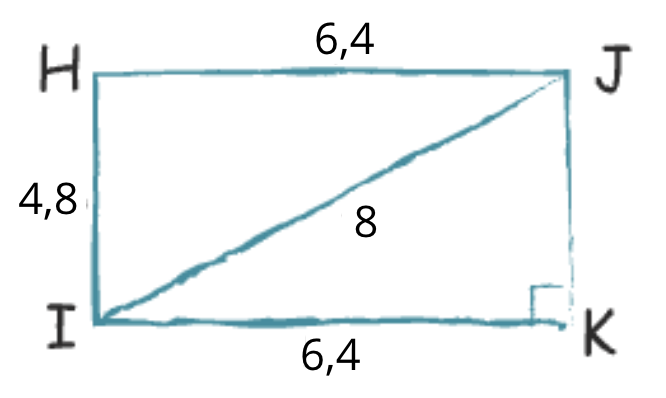
\includegraphics[scale=0.4]{exo1_1.png}
\end{center}
% \vspace{2pt}
Le quadrilatère obtenu est-il un rectangle ? Justifier avec \textbf{rigueur}.

\vspace{0.3cm}
\noindent\hrulefill
\vspace{1cm}

% % ---------------------------------------------------------
% \textbf{Exercice 2 – Nombres relatifs (6 points)}
% \vspace{5pt}
% \begin{questions}
%     \question[1] Calculer : $(-1) \times (-5) \times 2 \times (-7)
%     \times 10$
%     \question[1] Calculer :
%     \begin{parts}
%         \part $8 \times (-7)$
%         \part $(-0,2) \times 5$
%         \part $(-3)^3$
%         \part $(-3) : (-4)$
%         \part $-2^3$
%     \end{parts}
% \end{questions}

% \vspace{0.3cm}
% \noindent\hrulefill
% \vspace{1cm}

% ---------------------------------------------------------
\textbf{Exercice 2 – Distances (6 points)}
\vspace{5pt}

Calculer une valeur approchée au centimètre près de la distance entre
l'entrée de la résidence et l'entrée B du bâtiment.
\vspace{5pt}
\\\textbf{Justifier et détailler les calculs.}

\begin{center}
    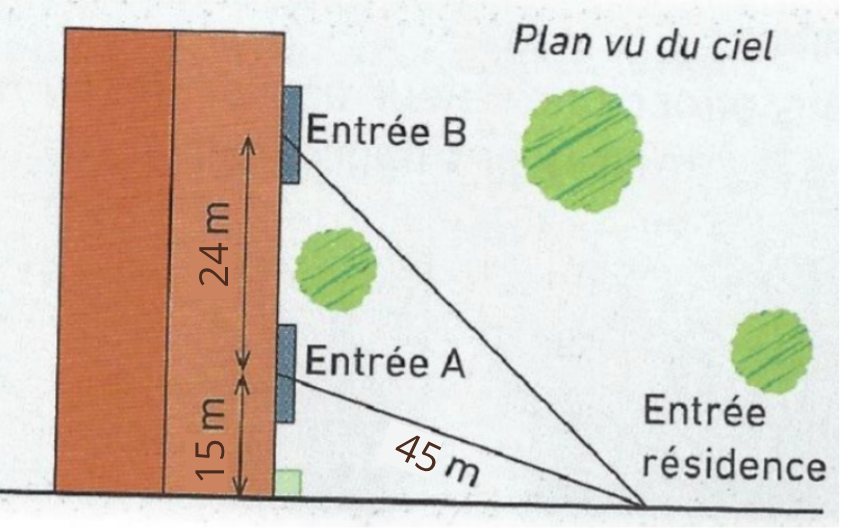
\includegraphics[scale=0.5]{exo3_2.png}
\end{center}

\vspace{0.3cm}
\noindent\hrulefill
\vspace{1cm}

% ---------------------------------------------------------
\textbf{Exercice 3 – Étude d'un triangle (4 points)}
\vspace{5pt}

$ABC$ est un triangle tel que $AB = 15\ mm$, $BC = 39\ mm$ et $AC = 36\ mm$.
\vspace{5pt}
\\
Le triangle $ABC$ est-il rectangle ? Justifier.

\vspace{0.3cm}
\noindent\hrulefill
\vspace{1cm}
\newpage
% ---------------------------------------------------------
\textbf{Exercice 4 – Calculs (6 points)}
\vspace{5pt}

\begin{questions}
    \question Déterminer le signe des opérations suivantes sans
    les calculer :
    \begin{parts}
        \part $A = (-8,2) \times 8 \times 1,75 \times (-3,7)$
        \part $B = \dfrac{-7}{-3,8 \times (-4,1)}$
    \end{parts}
    \question Effectuer les calculs suivants : 
    \begin{parts}
        \part $2 \times (-3) + 5 \times (-2) + 10 \times 2$
        \part $2 \times (8 - 4 \times 5) + 3$
        \part $-3^3$
        \part $(-8) : (-2)$
        \part $(-2)^3$
        \part $\dfrac{-3 \times 2 + 4}{-4+ 2 \times 3}$
    \end{parts}
\end{questions}

\vspace{0.3cm}
\noindent\hrulefill
\vspace{1cm}

% ---------------------------------------------------------
\textbf{Exercice BONUS – Énergie renouvelable (??? points)}
\vspace{5pt}

Pour produire une électricité plus propre, voilà le projet d'éolienne 
retenu par une ville dans l'Hérault.
\\Un ingénieur propose de la fixer sur un mât haubané. Il commande des câbles 
de $85\ m$ de long. Il installe une attache à un mètre du haut du pylône et relie 
cette attache au sol. Il veut fixer les câbles au sol à $13\ m$ de la base du mât. 
\\Il affirme qu'alors le mât sera bien perpendiculaire au sol.
\\
\vspace{5pt}\textbf{A-t-il raison ?}
\begin{center}
    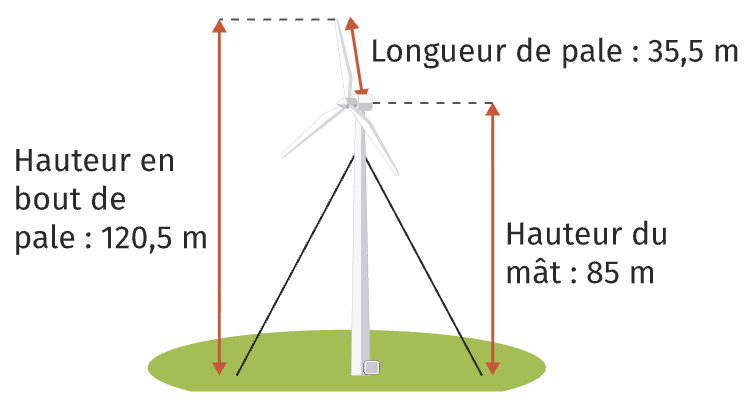
\includegraphics[scale=0.7]{exo_bonus.png}
\end{center}

\vspace{0.3cm}
\noindent\hrulefill
\vspace{1cm}


\vspace{0.5cm}
\begin{center}
\textbf{Fin du devoir — relire la copie avant de rendre.}
\end{center}

\end{document}
